\textbf{\underline{OZ 9 - Wisselstroomkringen - Oefening 3:}}
\vspace{0.5cm}

In de transformator is de weerstand in de belastingskring $R_L = 50.0 \ \Omega$. De verhouding van de windingen $\tfrac{N_1}{N_2} = \tfrac{5}{2}$, en de bronspanning is $80.0 \ \text{V}$ (rms). Als een voltmeter een belasting meet van $25.0 \ \text{V}$ (rms), wat is dan de bronweerstand $R_s$?

% \begin{enumerate}[(a)]
%     \item #
% \end{enumerate}

\begin{center}
    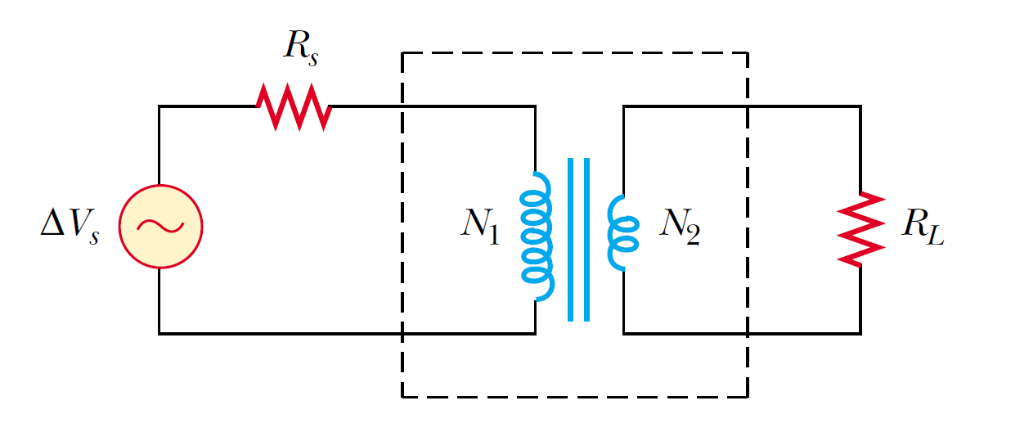
\includegraphics[scale = 0.4]{oz09/resources/Oz9Oef3.png}
\end{center}

\begin{description}[labelwidth=1.5cm, leftmargin=!]
    \item[Geg. :] $R_L = 50.0 \ \Omega$, $\tfrac{N_1}{N_2} = \tfrac{5}{2}$, $\Delta V_s = 80.0 \ \text{V}$, $\Delta V_L = 25.0 \ \text{V}$
    \item[Gevr. :]  $R_s$ ?
    \item[Opl. :]   
        We gebruiken de tweede wet van Kirchhoff voor de linker loop:
        \begin{equation*}
                \Delta V_s - I_sR_s - \mathcal{E}_1 = 0.
        \end{equation*}
        We weten dat
        \begin{align*}
            \mathcal{E}_1 &= \frac{N_1}{N_2}\Delta V_L = 62.5 \ \text{V} \\
            R_{eq} &= (\frac{N_1}{N_2})^2 R_L = 312.5 \ \Omega 
        \end{align*}
        en dus:
        \begin{equation*}
            R_s = \frac{\Delta V_s - \mathcal{E}_1}{\frac{\mathcal{E}_1}{R_{eq}}} = 87.5 \ \Omega.
        \end{equation*}
\end{description}

\vspace{1cm}